\chapter{Analisis}

\section{LSTM Autoencoder}

Data dipisah menjadi dua bagian, yaitu data normal yang mengandung data dari status NORMAL dan data anomali yang berasal dari status selain NORMAL (BROKEN dan RECOVERY).

Kemudian data dibagi menjadi 3 dataset, yaitu train, validation, dan test. Data train dan validation diambil pada bulan ke-8 awal dan akhir masing-masing dan digunakan untuk training model, sedangkan data test diambil pada selain bulan ke-8 untuk memprediksi hasil anomali.

Proses training model LSTM Autoencoder dilakukan sebanyak 5 epoch yang memakan waktu sekitar 20 menit. Data train dan validation dibagi menjadi dua macam, yaitu yang telah menggunakan PCA dan tanpa PCA.

Kemudian dilakukan prediksi pada data test dari model yang telah dilakukan training sehingga dapat diperoleh nilai loss yang dihasilkan.

    \subsection{Dengan PCA}

    \begin{figure}[h]
        \centering
        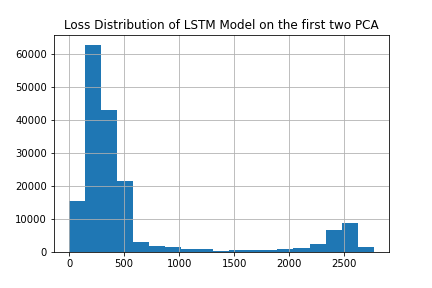
\includegraphics[width=0.8\textwidth]{resources/LSTM/LSTM_PCA_LossDist.png}
        \caption{Distribusi loss LSTM dengan PCA}
    \end{figure}

    Dengan menggunakan nilai threshold 500, diperoleh jumlah data anomali sebagai berikut.

    \begin{table}[h]
        \centering
        \begin{tabular}{|l|r|r|r|}
            \hline
            \multicolumn{1}{|c|}{\textbf{Jenis anomali}} & \multicolumn{1}{c|}{\textbf{Jumlah}} & \multicolumn{1}{c|}{\textbf{Total data}} & \multicolumn{1}{c|}{\textbf{Persentase (\%)}} \\ \hline
            Anomali pada data NORMAL                     & 33866                                & 160430                                   & 21                                       \\ \hline
            Anomali pada data selain NORMAL              & 2237                                 & 14454                                    & 15                                       \\ \hline
        \end{tabular}
    \end{table}

    Jumlah anomali pada data selain NORMAL tidak mencakup keseluruhan total data sehingga terdapat prediksi yang berada pada data dalam kondisi BROKEN atau RECOVERY.

    \subsection{Tanpa PCA}

    \begin{figure}[h]
        \centering
        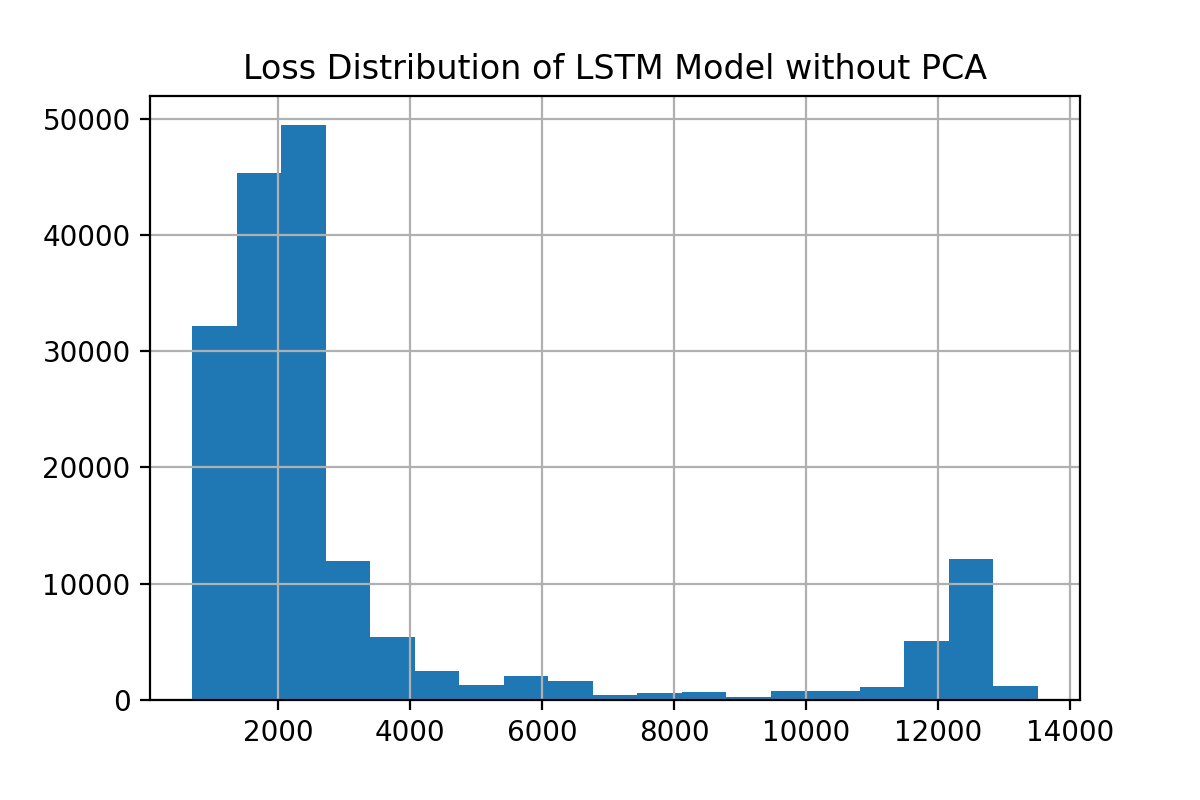
\includegraphics[width=0.8\textwidth]{resources/LSTM/LSTM_noPCA_LossDist.png}
        \caption{Distribusi loss LSTM tanpa PCA}
    \end{figure}

    Dengan menggunakan nilai threshold 3500, diperoleh jumlah data anomali sebagai berikut.

    \begin{table}[h]
        \centering
        \begin{tabular}{|l|r|r|r|}
            \hline
            \multicolumn{1}{|c|}{\textbf{Jenis anomali}} & \multicolumn{1}{c|}{\textbf{Jumlah}} & \multicolumn{1}{c|}{\textbf{Total data}} & \multicolumn{1}{c|}{\textbf{Persentase}} \\ \hline
            Anomali pada data NORMAL                     & 30182                                & 160430                                   & 19                                       \\ \hline
            Anomali pada data selain NORMAL              & 4979                                 & 14454                                    & 34                                       \\ \hline
        \end{tabular}
    \end{table}

    Terlihat bahwa jumlah anomali pada data NORMAL lebih sedikit 3\% dari analisis dengan PCA, Namun jumlah anomali pada data selain NORMAL juga meningkat hampir 2 kali lipat.
